

\section{DLRM Recommendation System Architecture}

To build a recommendation system based on a deep learning ranking model, there are several stages that the system should go through to provide the final recommendations.

Any system is a group of components that work together to achieve a goal according to a set of rules. The recommendation system is no different, it is a group of components that work together to provide personalized suggestions to users. There are two recommendation system types based on the number of stages they have:
\subsection{Two-stage Recommender Systems}
Two-stage recommender systems are systems that have two main stages as shown in figure \ref{fig:TwoStageRecSys}: candidate generation and ranking. The candidate generation stage is responsible for generating a set of candidate items for each user, while the ranking stage is responsible for ranking the candidate items and selecting the top items to be recommended to the user. The candidate generation stage is usually based on collaborative filtering or content-based filtering, while the ranking stage is usually based on ML models such as matrix factorization or deep learning models \cite{MultiStageRecSys}.
\begin{figure}[H]
    \centering
    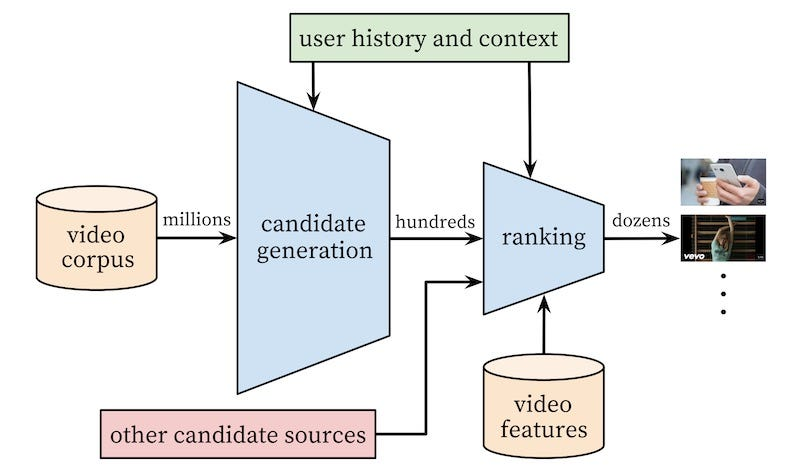
\includegraphics[width=0.6\textwidth]{assets/Two_stage_rec_sys.jpg}
    \caption[Two-stage Recommender System]{Two-stage Recommender System\cite{MultiStageRecSys}}
    \label{fig:TwoStageRecSys}
\end{figure}
\subsection{Four-stage Recommender Systems}
Four-stage recommender systems as shown in figure \ref{fig:FourStageRecSys} are systems that have four main stages: retrieval, filtering, scoring, and ordering. 
The retrieval stage is responsible for retrieving a set of candidate items for each user, 
the filtering stage is responsible for filtering the candidate items according to business rules and constraints,
and the ordering stage is responsible for ordering the scored items and selecting the top items to be recommended to the user. 
The retrieval stage is usually based on collaborative filtering or content-based filtering, while the filtering stage is 
usually based on ML models such as matrix factorization or deep learning models, and the scoring and ordering 
stages are usually based on ML models such as deep learning models \cite{NvidiaRecSysBestPractices}.
\begin{figure}[H]
    \centering
    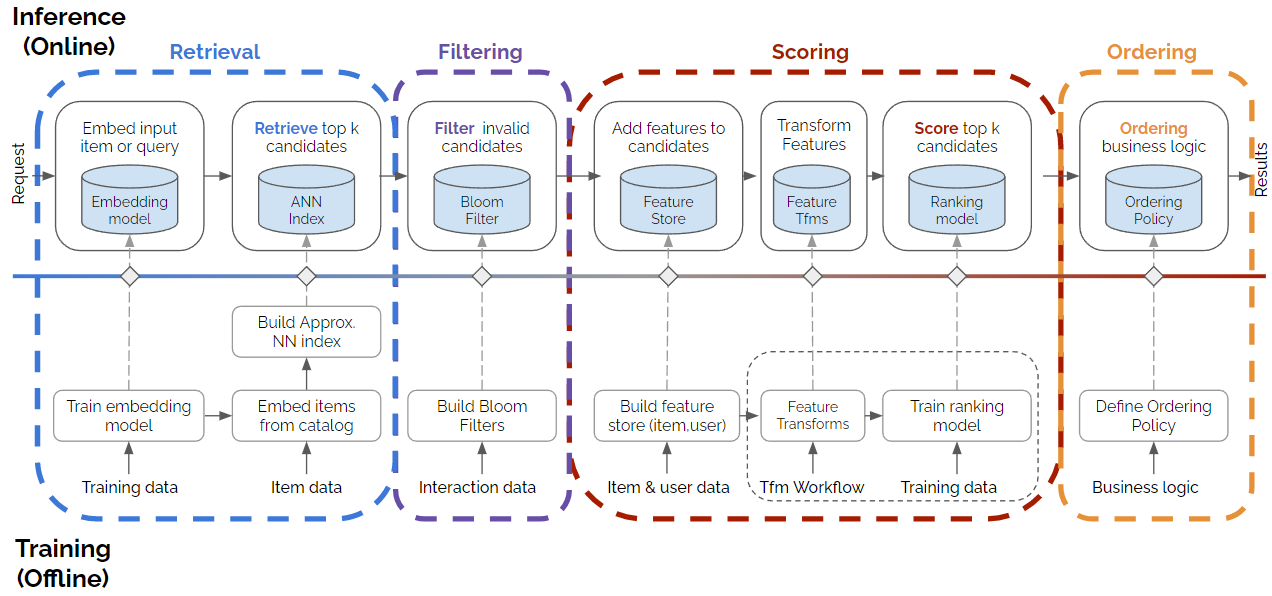
\includegraphics[width=1\textwidth]{assets/Four_stage_rec_sys.png}
    \caption[Four-stage Recommender System]{Four-stage Recommender System\cite{NvidiaRecSysBestPractices}}
    \label{fig:FourStageRecSys}
\end{figure}
each stage utilizes a set of components and algorithms in training and inference processes to achieve its goal.
\subsection{Dealing with categorical features}
One of the main challenges in building a recommendation system is dealing with high cardinality categorical features, which are features that have a large number of unique values. The high cardinality of categorical features makes it difficult to use traditional ML models such as linear regression and decision trees, as these models require the categorical features to be one-hot encoded, which results in a large number of features and a large model size. 
To deal with high cardinality categorical features, the DLRM uses several techniques such as:
\subsubsection{Features embedding}
Feature embedding is a technique used to represent categorical features as dense vectors of real numbers, where each unique value of the categorical feature is represented by a unique vector. The feature embedding technique is used to reduce the dimensionality of the categorical features and to learn the relationships between the unique values of the categorical features \cite{FeatureEmbedding}.
\subsubsection{Targaet encoding}
The target encoding technique is employed to encode categorical features with high cardinality by using the mean of the target variable for each unique value of the categorical feature. This technique helps reduce the dimensionality of the categorical features while encoding them based on their relationship with the target variable \cite{TargetEncoding}.
\subsection{Training (Offline)}
Like any ML system, the process of training the models occurs offline,
where the system is trained on a set of historical data, aka batched data, to optimize the model's parameters.
Also in the training phase, the system computes the feature embeddings for all users and items in addition to any other categorical features.


\subsection{Real-Time Inference (Online)}
The inference phase is when the system makes the predictions and suggestions for the application.
To be useful in any website or application, 
the system should be able to provide real-time predictions, 
and suggestions, with a few hundred milliseconds of latency.

In online inference, the system computes the recommendation in real-time based on the user's interactions and preferences, 
usually with user actions being the trigger for the recommendation generation process.

Figure \ref{fig:TwoStageOnline} shows a pipeline suggested by Nvidia\cite{NvidiaFeatureStores} for a two-stage online recommendation system.

\begin{figure}[H]
    \centering
    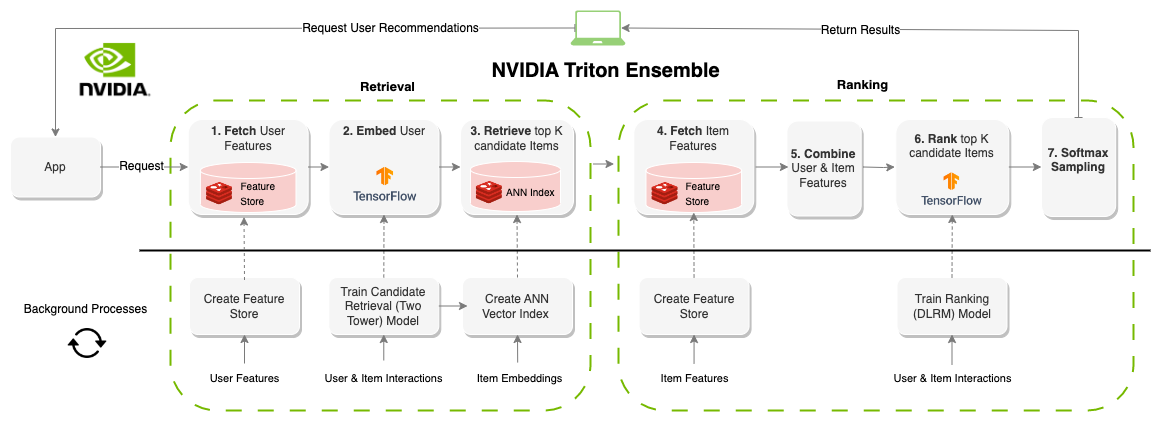
\includegraphics[width=1\textwidth]{assets/online-two-stage-recommender-pipeline.png}
    \caption[Two Stage Online Recommendation System]{Two Stage Online Recommendation System \cite{NvidiaFeatureStores}}
    \label{fig:TwoStageOnline}
\end{figure}



\subsection{Batch Inference (Offline)}
Unlike online inference, batch inference is the process of generating recommendations in advance and storing them, 
where the system computes the recommendations for all users and items, 
the process is repeated on a periodical basis.\cite{NvidiaFeatureStores} 
Figure \ref{fig:BatchRecSys} illustrates from a high perspective how a completely offline recommendation system operates.

This process allows much shorter response times and is useful for systems with a large number of users and items and a high volume of traffic.

Online and batched inference can be used together to provide real-time recommendations, where the system periodically pre-computes the recommendations for active users, but for new users, the system computes the recommendations in real-time.

\begin{figure}[H]
    \centering
    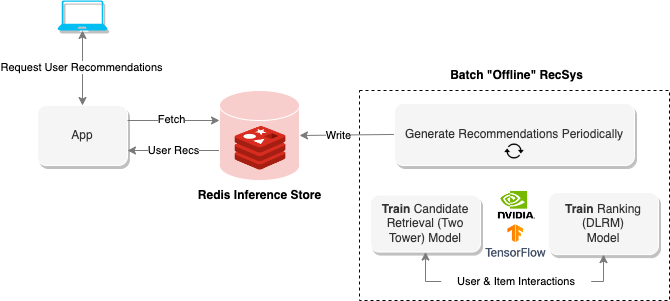
\includegraphics[width=1\textwidth]{assets/batch-recommendation-system.png}
    \caption[Batch Recommendation System]{Batch Recommendation System \cite{NvidiaFeatureStores}}
    \label{fig:BatchRecSys}
\end{figure}